\documentclass{beamer}
\usepackage{graphicx}
\usepackage{tikz}
\usetikzlibrary{shapes,arrows}
\usepackage{tikz}
\usetheme{default}
%\usecolortheme{seahorse}
  \setbeamertemplate{footline}[page number]
\usepackage{multirow}
\setbeamertemplate{navigation symbols}{}
\setbeamertemplate{frametitle}[default][center]
\setbeamerfont{frametitle}{shape=\scshape}

\usepackage{xcolor}

\usepackage[flushleft]{threeparttable}

{\title{\textsc{Markov Chain Monte Carlo, Numerical Integration} \\ \tiny (See Statistics)}
\author{Trevor Gallen}
\date{}
\begin{document}
\renewcommand*{\inserttotalframenumber}{\pageref{lastframe}}

\begin{frame}
\titlepage
\end{frame}


\begin{frame}
\frametitle[alignment=center]{Agenda}
\begin{itemize}
\item Numerical Integration: MCMC methods
\bigskip
\item Estimating Markov Chains 
\bigskip
\item Estimating latent variables
\end{itemize}
\end{frame}

\begin{frame}
\frametitle[alignment=center]{Numerical Integration: Part II}
\begin{itemize}
\item Quadrature for one to a few dimensions feasible for well-behaved distributions
\bigskip
\item For many-dimensional integrals, we typically use Markov chain Monte Carlo
\bigskip
\item There are many different methods
\bigskip
\item I discuss a simple one (Gibbs Sampling) and a more complex one (Metropolis-Hastings)
\bigskip
\item This is a prominent problem in Bayesian analysis
\end{itemize}
\end{frame}

\begin{frame}
\frametitle[alignment=center]{The Problem}
\begin{itemize}
\item Say your data is summarized by a two-dimensional problem: height and weight $f(x_1,x_2)$
\bigskip
\item You want a population, for $i\in(1,...,n)$,  $(x_1^{i},x_2^{i})$
\bigskip
\item You have access to the \emph{conditional} marginal distributions.  That is, while $f(x_1,x_2)$ is ugly, 
$f(x_1|x_2)$ and $f(x_2|x_1)$ are easy to sample from.  
\end{itemize}
\end{frame}

\begin{frame}
\frametitle[alignment=center]{Gibbs Sampling}
\begin{enumerate}
\item Start with $(x_1^0,x_2^0)$
\bigskip
\item Sample $x_1^{1}\sim f(x_1|x_2^0)$
\bigskip
\item Sample $x_2^{1}\sim f(x_2|x_1^1)$
\bigskip
\item We have a LLN and CLT that states that:
$$\frac{1}{N}\sum_{i=1}^Ng(x^{i})\rightarrow \int g(x)f(x)dx$$
\end{enumerate}
\end{frame}

\begin{frame}
\frametitle[alignment=center]{Gibbs Sampling: Example}
\begin{itemize}
\item Assume a distribution:
$$x\sim\mathcal{N}\left(0,\Sigma\right)\ \ \ \Sigma=\left[\begin{array}{cc}1 & \rho \\ \rho & 1\end{array}\right]$$
\item Then we can get the conditional marginal distributions:
$$x_1|x_2\sim\mathcal{N}\left(\rho x_2,(1-\rho)^2\right)$$
$$x_2|x_1\sim\mathcal{N}\left(\rho x_1,(1-\rho)^2\right)$$
\item Iteratively sample from these.
\bigskip
\item See Gibbs.m
\end{itemize}
\end{frame}

\foreach \x in {1,2,...,20}
{
\begin{frame}
\frametitle[alignment=center]{Gibbs Sampling: Example}
\includegraphics[scale=0.5]{Gibbs_\x.png}
\end{frame}
}

\begin{frame}
\frametitle[alignment=center]{Metropolis Hastings}
What if we can only evaluate likelihood at a given point?
\begin{enumerate}
\bigskip
\item We start with some (multi-dimensional) value $x^{i}$ and a proposal distribution $g(x|x^{i})$
\bigskip
\item Grab a new sample from our proposal distribution:
$$x'\sim g(x|x^i)$$
\item Calculate acceptance probability:
$$pr(x^i,x')=\min\left\{1,\frac{f(x')}{f(x^i)}\frac{g(x^i|x')}{g(x',x^i)}\right\}$$
\item Accept the new value with probability $pr(x^i,x')$, otherwise, stay there.
\bigskip
\item This again converges in distribution to the true distribution.
\end{enumerate}
\end{frame}

\begin{frame}
\frametitle[alignment=center]{A convenient proposal density}
\begin{itemize}
\item If our proposal density is symmetric
$$g(x^i|x')=g(x',x^i)$$
\item This is called random-walk Metropolis-Hastings
\bigskip
\item Our acceptance probability is easy:
$$pr(x^i,x')=\min\left\{1,\frac{f(x')}{f(x^i)}\right\}$$
\end{itemize}
\end{frame}

\begin{frame}
\frametitle[alignment=center]{Metropolis-Hastings: Example}
\begin{itemize}
\item Let's say our distribution is one-dimensional:
$$x\sim0.5U(0,1)+0.25U(-1,2)+0.25U(0.5,0.75)$$
\item Choose sampling distribution centered around current point:
$$g(x'|x)\sim\mathcal{N}(x,0.1)$$
\end{itemize}
\end{frame}

\begin{frame}
\frametitle[alignment=center]{Sampling PDF}
\begin{itemize}
\item Let's say our distribution is one-dimensional:
$$x\sim0.5U(0,1)+0.25U(-1,2)+0.25U(0.5,0.75)$$
\item Choose sampling distribution centered around current point:
$$g(x'|x)\sim\mathcal{N}(x,0.1)$$
\end{itemize}
\end{frame}

\foreach \x in {1,2,...,30}
{
\begin{frame}
\frametitle[alignment=center]{Metropolist-Hastings Random Walk: Example}
\includegraphics[scale=0.5]{MH_\x.png}
\end{frame}
}

\begin{frame}
\frametitle[alignment=center]{Sampling PDF}
\begin{itemize}
\item Let's say our distribution is one-dimensional:
$$x\sim0.5U(0,1)+0.25U(-1,2)+0.25U(0.5,0.75)$$
\item Choose sampling distribution centered around current point:
$$g(x'|x)\sim\mathcal{N}(x,0.1)$$
\end{itemize}
\end{frame}

\begin{frame}
\frametitle[alignment=center]{Why learn MH \& Numerical Integration?}
\begin{itemize}
\item Many-dimensional problems
\bigskip
\item Bayesian estimation
\bigskip
\begin{itemize}
\item Write down model
\bigskip
\item Write down distribution of parameters $f(\theta)$
\bigskip
\item Simulate many models to get model distribution of data $f(x|\theta)$
\bigskip
\item Update your beliefs: $f(\theta|x)\propto f(\theta)f(x|\theta)$
\end{itemize}
\item Typically need to draw from posterior distribution without an analytical calculation
\bigskip
\item Use M-H
\end{itemize}
\end{frame}

\begin{frame}
\frametitle[alignment=center]{Metropolis-Hasting Example-Motivation}
\begin{itemize}
\item Consider a human capital accumulation problem (as in Homework 1, 2 in 2023)
\bigskip
\item Households choose how much time to study vs. work, no asset accumulation
\bigskip
\item VFI problem, but want to estimate depreciation rate and ability level
\bigskip
\item Bayesian Structural Estimation!
\end{itemize}
\end{frame}

\begin{frame}
\frametitle[alignment=center]{Model/Problem}
$$V(h)=\underset{i}{\max}\left\{log((1-i)h)+\beta V((1-\color{red}{\delta}\color{black})h+\color{red}{A}\color{black}i^\gamma)\right\}$$
\begin{itemize}
\bigskip
\item Where \textcolor{red}{$A$}, \textcolor{red}{$\delta$} are to be estimated from decision data in the problem ($\gamma$ is known).
\bigskip
\item For convenience (real structural problem would have more natural probabilities), $i^{obs}=i^{data}+\epsilon$ where $\epsilon\sim\mathcal{N}\left(0,\sigma^2\right)$
\bigskip
\item For convenience, I solve this for a grid of $\delta$ and $A$
\bigskip
\item This gives me pr(data|parameter)
\bigskip
\item Metropolis-Hastings lets me combine model based probability p(parameter) to get p(parameter|data) without having to integrate across
\end{itemize}
\end{frame}

\begin{frame}
\frametitle[alignment=center]{Model}
\begin{itemize}
\item Assume prior distribution of $\{A,\delta\}$ (here independently distributed $f(A)\sim\mathcal{N}(1,0.05)$ $f(\delta)\sim\mathcal{U}(0.03,0.08)$
\item Use transition distribution $\Delta\theta\sim\mathcal{N}(0,0.01)$
\item Have probability of choice conditional on parameter $g(i|\theta)$  from structural model
\item Have starting point for MCMC $\theta_0\sim\mathcal{N}(1,0.05) $
\begin{itemize}
\item Draw new $\theta_1=\theta_0+\Delta\theta$
\item Compare: $r=\frac{g(i|\theta_1)f(\theta_1)}{g(i|\theta_0)f(\theta_0)}$
\item Either accept or reject based on MH algo
\item Repeat many times
\item Now have sampling from posterior distribution
\end{itemize}
\item See Main.m, VFIGridSolver.m, and MCMC.m
\end{itemize}
\end{frame}

\begin{frame}
\frametitle[alignment=center]{Model}
\begin{figure}
\centering
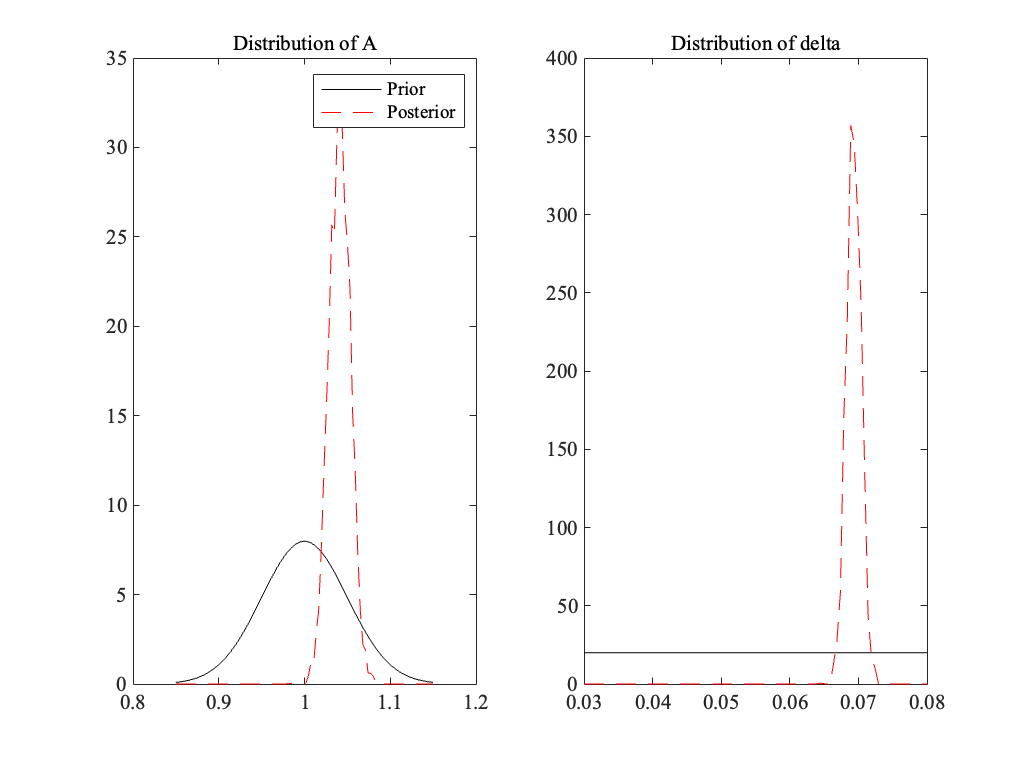
\includegraphics[scale=0.3]{MCMC_Example_VFI.png}
\end{figure}
\end{frame}


\begin{frame}
\frametitle[alignment=center]{Aside:  Multiple Hypothesis Testing and Maximum F-Statistics}
\begin{itemize}
\item Data is tortured.  When you see...
\bigskip
\begin{itemize}
\item ..an experiment with multiple test groups or with without very strong theoretical justification, be skeptical!
\smallskip
\item ...a regression that could have been run differently, or with many potential controls, weighting options, and unit-of-observation choices, be skeptical!
\smallskip
\end{itemize}
\item Not all bad: t-statistics might just be heuristics...when I see 0.01 in a regression where I could imagine 10 other setups, I know the real p-value is around 0.1.
\bigskip
\item But we might want to take statistics seriously, or data-mine honestly
\bigskip
\item We can simulate the distribution of the maximum F-statistic, or the maximum t-statistic.
\bigskip
\item See MonteCarlo.do and similar exercises (Note: Stata!)
\end{itemize}
\end{frame}




\end{document}